%!TEX TS-program = xelatex

%%%%%%%%%%%%%%%%%%%%%%%%%%%%%%%%%%%%%%%%%%%%%%%%
% CV template
% Originally created by Adrien Friggeri
% Improved by Carmine Benedetto
%%%%%%%%%%%%%%%%%%%%%%%%%%%%%%%%%%%%%%%%%%%%%%%%

\documentclass[]{cv-class}
\usepackage{afterpage}
\usepackage{hyperref}
\usepackage{color}
\usepackage{xcolor}
\hypersetup{
    colorlinks=true,
    linkcolor=blue
}
\RequirePackage{xcolor}
\definecolor{pblue}{HTML}{0395DE}

\begin{document}
\header{Rohit}{Kumar}
     % {Data Science Practitioner}
      {Big Data and Data Science Practitioner}

% Fake text to add separator
\vspace{1.15cm}
\fcolorbox{white}{gray}{\parbox{\dimexpr\textwidth-2\fboxsep-2\fboxrule}{%
.....
}}

% In the aside, each new line forces a line break
\begin{aside}
  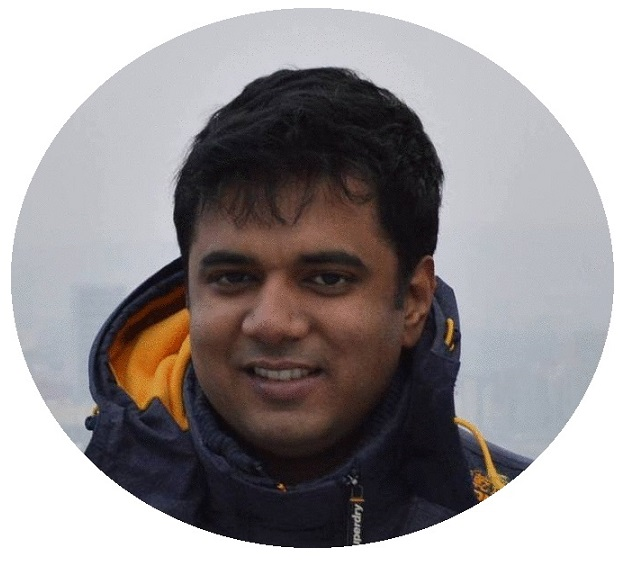
\includegraphics[scale=0.30]{img/meg2.jpg}
    ~
  \vspace{0.65cm}
%  \section{Civil status}
%    Married
%  	~
  \section{Address}
    Avenue General Medicine Derache 28\\
    Brussels 1050\\
    Belgium
    ~
  \section{Phone}
    +32 465 931 350
    ~
  \section{Mail}
    \underline{\href{mailto:rohit1308k@gmail.com}{rohit1308k@gmail.com}}
	%	 \underline{\href{mailto:rohitkumar@exadive.com}{rohitkumar@exadive.com}}
    ~
  %\section{Web}
 %	\vspace{0.10cm}
%    \underline{\href{https://www.linkedin.com/in/rohit13k/}{linkedin.com/in/rohit13k/}}
	%\vspace{0.10cm}
  %  \underline{\href{rohit13k.github.io}{rohit13k.github.io}}
%	\vspace{0.10cm}
 %\underline{\href{https://github.com/rohit13k}{github.com/rohit13k}}
    ~
  \section{Programming}
    \asidelist{\textbf{Java}}
    {
\includegraphics[scale=0.30]{img/star.png}
    
\includegraphics[scale=0.30]{img/star.png}
    
\includegraphics[scale=0.30]{img/star.png}
    
\includegraphics[scale=0.30]{img/star.png}
    
\includegraphics[scale=0.30]{img/star.png}}
    \asidelist{\textbf{Scala}}
    {
\includegraphics[scale=0.30]{img/star.png}
    
\includegraphics[scale=0.30]{img/star.png}
    
\includegraphics[scale=0.30]{img/star.png}
    
\includegraphics[scale=0.30]{img/star.png}
    
\includegraphics[scale=0.30]{img/star_empty.png}}
    \asidelist{\textbf{R}}
    {
\includegraphics[scale=0.30]{img/star.png}
    
\includegraphics[scale=0.30]{img/star.png}
    
\includegraphics[scale=0.30]{img/star.png}
    
\includegraphics[scale=0.30]{img/star_empty.png}
    
\includegraphics[scale=0.30]{img/star_empty.png}}
    \asidelist{\textbf{Python}}
    {
\includegraphics[scale=0.30]{img/star.png}
    
\includegraphics[scale=0.30]{img/star.png}
    
\includegraphics[scale=0.30]{img/star.png}
    
\includegraphics[scale=0.30]{img/star_empty.png}
    
\includegraphics[scale=0.30]{img/star_empty.png}}
      ~
  \section{Databases}
    \asidelist{\textbf{MySQL}}
    {
\includegraphics[scale=0.30]{img/star.png}
    
\includegraphics[scale=0.30]{img/star.png}
    
\includegraphics[scale=0.30]{img/star.png}
    
\includegraphics[scale=0.30]{img/star.png}
    
\includegraphics[scale=0.30]{img/star.png}}
    \asidelist{\textbf{MS SQL}}
    {
\includegraphics[scale=0.30]{img/star.png}
    
\includegraphics[scale=0.30]{img/star.png}
    
\includegraphics[scale=0.30]{img/star.png}
    
\includegraphics[scale=0.30]{img/star_empty.png}
    
\includegraphics[scale=0.30]{img/star_empty.png}}
    \asidelist{\textbf{Oracle Coherence}}
    {
\includegraphics[scale=0.30]{img/star.png}
    
\includegraphics[scale=0.30]{img/star.png}
    
\includegraphics[scale=0.30]{img/star_empty.png}
    
\includegraphics[scale=0.30]{img/star_empty.png}
    
\includegraphics[scale=0.30]{img/star_empty.png}}
   
        ~
        \section{Big Data Systems}
    \asidelist{\textbf{Spark}}
    {
\includegraphics[scale=0.30]{img/star.png}
    
\includegraphics[scale=0.30]{img/star.png}
    
\includegraphics[scale=0.30]{img/star.png}
    
\includegraphics[scale=0.30]{img/star.png}
    
\includegraphics[scale=0.30]{img/star.png}}
    \asidelist{\textbf{Hadoop}}
    {
\includegraphics[scale=0.30]{img/star.png}
    
\includegraphics[scale=0.30]{img/star.png}
    
\includegraphics[scale=0.30]{img/star.png}
    
\includegraphics[scale=0.30]{img/star_empty.png}
    
\includegraphics[scale=0.30]{img/star_empty.png}}
    \asidelist{\textbf{Flink}}
    {
\includegraphics[scale=0.30]{img/star.png}
    
\includegraphics[scale=0.30]{img/star.png}
    
\includegraphics[scale=0.30]{img/star_empty.png}
    
\includegraphics[scale=0.30]{img/star_empty.png}
    \includegraphics[scale=0.30]{img/star_empty.png}}
    ~
     \asidelist{\textbf{Kafka}}
    {\includegraphics[scale=0.30]{img/star.png}
    \includegraphics[scale=0.30]{img/star.png}
    \includegraphics[scale=0.30]{img/star_empty.png}
    \includegraphics[scale=0.30]{img/star_empty.png}
    \includegraphics[scale=0.30]{img/star_empty.png}}
    ~
     \asidelist{\textbf{NoSQL}}
    {\includegraphics[scale=0.30]{img/star.png}
    \includegraphics[scale=0.30]{img/star.png}
    \includegraphics[scale=0.30]{img/star_empty.png}
    \includegraphics[scale=0.30]{img/star_empty.png}
    \includegraphics[scale=0.30]{img/star_empty.png}}
    
\end{aside}

\vspace{0.75cm}
\section{Experience}
\begin{entrylist}
 % \entry
 %   {Aug. 14 - Now}
  %  {PhD Researcher}
   % {Universit\'{e} Libre de Bruxelles (ULB), Belgium}
   % {
	
    %Expected, a Ph.D. in ``Graph Data stream mining and distributed processing" in June 2018 from ULB (Brussels) and UPC (Barcelona). The research focuses on designing efficient one pass algorithms to analysis large interaction networks such as social media network.\\
  %   Worked on social network analysis and viral marketing.\\
    %  Currently, working on distributed graph processing on Apache Spark GraphX. 
     % Worked on other Distributed processing systems like Hadoop, MongoDB, Kafka, Hive and Cassandra. 
		%	Worked on large graph querying and processing using Giraph, Apache GraphX and Neo4j.\\
		%	Teaching/Lab assistant for data-warehouse course for one semester for a class of 20 master students.
   %   1 A* rank, 2 A rank and 1 B rank full conference papers published.
    
    %}
  \iffalse
\entry
    {Sep. 17 - Now}
    {Online Corporate Trainer (Freelance)}
    {Digital Vidya, India}
    { Designed and delivered online course on Big Data Engineering course (Hadoop, Spark, Hive, Pig, Cassandra, NoSQL) for Digital Vidya for a batch of 10 students.\\
 Delivered online course on Data science with Python (NumPy, Pandas, scikit-learn) and Scala (Spark Mllib) for Digital Vidya online courses. \\}
  \entry
    {Sep. 16 - Oct. 16}
    {Data Engineer (Freelance)}
    {Disperse.io, UK}
    { Worked on analyzing and discovering trends in Wi-Fi data for London metro stations. Worked as freelance data engineer in data cleaning and data analysis using Spark-SQL. \\}
		\fi
\entry
    {Aug. 14 - now}
    {Big Data Scientist (Freelance)}
    {Upwork}
    { Worked on multiple short and long term projects for multiple clients on big data and data science domain.\\
			- Disperse.io: Worked on analyzing and discovering trends in Wi-Fi data for London metro stations. Worked as data engineer in data cleaning and data analysis using Spark-SQL.\\
			- Discovergy: Worked on smart meter applications. Developed a machine learning based platform on top of Spark streaming to collect, store and analysis data from smart meters. \\
			- L3Networks: Designed and implemented a processing system that could process web logs arriving at the rate of 46GB/min in real-time. Designed the architecture and the data processing pipeline using Apache Kafka, Apache Spark and Apache Hadoop using Java and Scala Languages. The work included deployment of these technologies as well.\\
			- DigitalVidya: Designed and delivered online course on Big Data Engineering course (Hadoop, Spark, Hive, Pig, Cassandra, NoSQL) for DigitalVidya for 3 batches of 10 students. Currently delivering a course on Data Science with Python (NumPy, Pandas, scikit-learn) and R.\\
			}		
 \entry
    {Jun. 14 - Jul. 14}
    {Software Designer}
    {Royal bank of Scotland, Delhi, India}
    {Developed data pipelines for the massive amount of banking and trading data for RBS using in-memory database on Oracle Coherence. \\}
  \entry
    {Apr. 11 - May. 14}
    {Assistant Consultant}
    {Tata Consultancy Services, Mumbai, India}
    {Technical team lead and Scrum Master for the entire online assessment platform, an online cloud based system for conducting online examinations and certifications. As technical lead I was responsible for 10 different products on the assessment platform and was supervising a team of 30 developers.\\
		I was the lead architect and developer for the deployment of the complete rco-system of the online assessment platform in multi-tenant architecture for software as a service model. I also contributed as technical expert in pre sales and helped in designing new product offerings for the education domain. \\
    Technologies used: J2EE, Java, MySQL, SVN, Struts 2, Hibernate, Memcached, Adobe Flex\\}
  \entry
    {Mar. 11 - Sep. 11}
    {Researcher}
    {Tata Research Development and Design Center, Pune, India}
    {Worked on data privacy and data security. Worked on data masking techniques for privacy preserving data mining. \\
     Technologies used: C++, CVS\\}

\end{entrylist}
\newpage

\begin{entrylist}
  \entry
    {Nov. 07 - Mar. 11}
    {Assistant System Engineer}
    {Tata Consultancy Services, Chennai, India}
    {Lead architect to develop and deploy the online assessment platform for TCS hiring throughout India. 
 Performance and Security Lead for the online assessment platform. Taught Algorithms and Java to new employees as a part of learning and development program.\\
  Technologies used: Java, CVS, Haskel, Java Security library, MS SQL.\\}
  \entry
    {Jun. 05 - Jun. 07}
    {Summer Research Intern}
    {JNCSAR, IISC, Bangalore, India}
    {
    Did two summer(2 months) and one winter(1 month) research internship in Nanoscience.
    Worked with P.hD students on analyzing nano material properties under electron microscopes.\\}
\end{entrylist}


\section{Education}
\begin{entrylist}
  \entry
    {Aug. 14 - Now}
    {Ph.D Candidate}
    {Universit\'{e} Libre de Bruxelles \&  Universitat Polit\'{e}cnica de Catalunya}
   % {Doing a joint PhD from ULB and UPC under joint supervision from Toon Calders and Alberto Abello, Funded by FNRS scholarship.\\}
	{Doing PhD from ULB on Graph Stream mining and distributed processing.}
  \entry
    {Aug. 08 - Apr. 11}
    {M.Sc in Computer Science}
    {Chennai Mathematical Institute, India}
    {The Master course was done part time while working in TCS.
    Main subjects: Discreet Mathematics, Database Systems, Operating systems, Data mining, Cryptography, Statistics, Design and Analysis of Algorithm,
    Theory of Computation, Programming language Concepts. Grade: \textbf{8.44\%}\\
    Thesis: Security aspects of online Assessment platform-Touchstone.\\}
      \entry
    {Jul. 04 - Jul. 07}
    {B.Sc (Hons) in Physics}
    {Hindu College, Delhi University}
    {Did summer research internship at IISC Bangalore every summer break. Co-Organized Physics Department fest on 2006.
     Percentage: \textbf{76.1\%}\\}
\end{entrylist}


\begin{aside}
  \vspace{1cm}
  \section{Languages}
    \asidelist{\textbf{English}}
    {\includegraphics[scale=0.30]{img/star.png}
    \includegraphics[scale=0.30]{img/star.png}
    \includegraphics[scale=0.30]{img/star.png}
    \includegraphics[scale=0.30]{img/star.png}
    \includegraphics[scale=0.30]{img/star.png}}
    \asidelist{\textbf{Hindi}}
    {\includegraphics[scale=0.30]{img/star.png}
    \includegraphics[scale=0.30]{img/star.png}
    \includegraphics[scale=0.30]{img/star.png}
    \includegraphics[scale=0.30]{img/star.png}
    \includegraphics[scale=0.30]{img/star.png}}
    \asidelist{\textbf{Spanish}}
    {\includegraphics[scale=0.30]{img/star.png}
    \includegraphics[scale=0.30]{img/star_empty.png}
    \includegraphics[scale=0.30]{img/star_empty.png}
    \includegraphics[scale=0.30]{img/star_empty.png}
    \includegraphics[scale=0.30]{img/star_empty.png}}
    ~
   \section{Personal Skills}
    \includegraphics[scale=0.20]{img/personal.png}
    ~
\end{aside}

\section{Awards and Achievements}
\begin{entrylist}
  \entry
    {Apr. 13}
    {Best Technical Lead Award in ACTion2013 in SMB iON}
    {TCS}
    {Awarded best technical lead in the entire department of 500 developers and 25 teams.\\}
      \entry
    {Sep. 11}
    {Innovation of the year award southern region}
    {Tata Innovista}
    {Tata group yearly award for innovations across the Tata groups  companies.\\}
   
\end{entrylist}

\section{Publications}
\begin{entrylist}
	\entry
	{2017}
	{Activity-Driven Influence Maximization in Social Networks}
	{ECML/PKDD}
	{\textbf{Rohit Kumar}, Muhammad Aamir Saleem, Toon Calders, Xike Xie and Torben Bach Pedersen\\}
	\entry
	{2017}
	{Cost Model for Pregel on GraphX}
	{ADBIS}
	{\textbf{Rohit Kumar}, Alberto Abello, and Toon Calders\\}
		\entry
	{2017}
	{Information Propagation in Interaction Networks.}
	{EDBT}
	{\textbf{Rohit Kumar} and Toon Calders\\}
		
	\end{entrylist}
	\begin{entrylist}
	\entry
	{2017}
	{Location Influence in Location-based Social Networks.}
	{WSDM}
	{Muhammad Aamir Saleem, \textbf{Rohit Kumar}, Toon Calders, Xike Xie and Torben Bach Pedersen\\}
	\entry
	{2017}
	{Finding simple temporal cycles in an interaction network.}
	{TD-LSG}
	{\textbf{Rohit Kumar} and Toon Calders\\}
	\entry
	{2017}
	{IMaxer: A Unified System for evaluating Influence Maximization Mechanisms in Location-based Social Networks}
	{CIKM}
	{Muhammad Aamir Saleem, \textbf{Rohit Kumar}, Toon Calders, Xike Xie and Torben Bach Pedersen\\}
	\entry
	{2017}
	{Cost Model Based Approach for Graph Partitioning in Spark GraphX}
	{DBDBD}
	{\textbf{Rohit Kumar}, Alberto Abello, and Toon Calders\\}
	\entry
	{2015}
	{Maintaining sliding-window neighborhood profiles in interaction networks.}
	{ECML/PKDD}
	{\textbf{Rohit Kumar}, Toon Calders, Aristides Gionis, and Nikolaj Tatti.\\}
	\end{entrylist}
	\section{Patents}
	\begin{entrylist}
	\entry
	{2009}
	{System and method for automated competency assessment}
	{US8915744}
	{Raman Srinivasan, Priyadharshini Sridhar, Swarna Srinivasan, \textbf{Rohit Kumar}, Radhika Jayapaul, Radhika Ganesan, Amit Nath, Vikash Agarwal}
	\entry
	{2013}
	{Customized question paper generation}
	{US20130084554A1}
	{Viral Prakash SHAH, Nawaz Shaikh,\textbf{ Rohit Kumar}}
	\entry
	{2014}
	{Secured Computer Based Assessment}
	{US20140186812A1}
	{Viral Prakash SHAH, Nawaz Shaikh,\textbf{ Rohit Kumar}}
	\end{entrylist}

\vspace{1.5cm}
\begin{flushright}
\emph{Rohit Kumar}
\end{flushright}
\begin{flushright}
\emph{\today}
\end{flushright}

\end{document}
